% !TEX program = pdflatex
% FRE6883 Recitation 1 -- C++ Survival Kit
\documentclass[10pt,aspectratio=169]{beamer}

% Language & encoding
\usepackage[utf8]{inputenc}
\usepackage[T1]{fontenc}
\usepackage[english]{babel}
\usepackage{lmodern}
\usepackage{microtype}
\DisableLigatures{encoding=*,family=tt*}

% Math / tables / layout
\usepackage{amsmath,amssymb,bm,mathtools}
\usepackage{booktabs}
\usepackage{multicol}
\usepackage{changepage}

% Graphics
\usepackage{graphicx}
\usepackage{tikz}
\usetikzlibrary{arrows.meta,positioning,calc,decorations.pathreplacing}
\usepackage{pgfplots}
\pgfplotsset{compat=1.18}

% Theme (Metropolis)
\usetheme[numbering=fraction,progressbar=frametitle]{metropolis}
\setbeamertemplate{frame numbering}[fraction]
\setbeamertemplate{navigation symbols}{}

% Bootcamp palette
\definecolor{BootcampBlueDark}{HTML}{1A3C68}
\definecolor{BootcampBlue}{RGB}{31,110,178}
\definecolor{AccentGold}{HTML}{DAA520}
\definecolor{SoftGray}{RGB}{245,246,248}
\definecolor{TextBlack}{HTML}{000000}
\definecolor{Crimson}{HTML}{990000}
\definecolor{MatrixGreen}{HTML}{228B22}
\definecolor{MatrixRed}{HTML}{B22222}

% Global formatting
\setbeamercolor{normal text}{fg=TextBlack,bg=white}
\setbeamercolor{title}{fg=TextBlack}
\setbeamercolor{structure}{fg=BootcampBlueDark}
\setbeamercolor{progress bar}{fg=BootcampBlueDark,bg=gray!30}

\setbeamercolor{frametitle}{bg=BootcampBlueDark,fg=white}
\setbeamerfont{frametitle}{series=\bfseries,size=\large}
\setbeamertemplate{frametitle}{
  \nointerlineskip
  \begin{beamercolorbox}[wd=\paperwidth,ht=3.2ex,dp=1.4ex,leftskip=1em,rightskip=1em]{frametitle}
    \usebeamerfont{frametitle}\insertframetitle
  \end{beamercolorbox}
}

\setbeamercolor{block title example}{bg=BootcampBlueDark!90!black,fg=white}
\setbeamercolor{block body example}{bg=BootcampBlueDark!5!white,fg=black}
\setbeamercolor{block title proposition}{bg=MatrixGreen!75!black,fg=white}
\setbeamercolor{block body proposition}{bg=MatrixGreen!7!white,fg=black}
\setbeamercolor{block title illustration}{bg=AccentGold!85!black,fg=white}
\setbeamercolor{block body illustration}{bg=AccentGold!10!white,fg=black}
\setbeamercolor{block title proof}{bg=gray!70!black,fg=white}
\setbeamercolor{block body proof}{bg=SoftGray,fg=black}
\setbeamertemplate{blocks}[rounded][shadow=false]

\newenvironment{definitionblock}[1]{%
  \par\vspace{0.4em}%
  \begin{beamercolorbox}[
      wd=\textwidth,sep=0.4em,leftskip=0.3em,rightskip=0.6em,
      rounded=false,shadow=false
    ]{block title example}%
    \raisebox{0.15em}{\usebeamerfont{block title example}#1}%
  \end{beamercolorbox}%
  \vspace{-0.4em}%
  \begin{beamercolorbox}[
      wd=\textwidth,sep=0.9em,leftskip=0.6em,rightskip=0.6em,
      rounded=false,shadow=false
    ]{block body example}%
    \usebeamerfont{block body example}%
}{%
  \end{beamercolorbox}%
  \par\vspace{0.6em}%
}

\newenvironment{propositionblock}[1]{%
  \par\vspace{0.35em}%
  \begin{beamercolorbox}[
      wd=\textwidth,sep=0.4em,leftskip=0.3em,rightskip=0.6em,
      rounded=false,shadow=false
    ]{block title proposition}%
    \raisebox{0.15em}{\usebeamerfont{block title example}#1}%
  \end{beamercolorbox}%
  \vspace{-0.4em}%
  \begin{beamercolorbox}[
      wd=\textwidth,sep=0.8em,leftskip=0.6em,rightskip=0.6em,
      rounded=false,shadow=false
    ]{block body proposition}%
    \usebeamerfont{block body example}%
}{%
  \end{beamercolorbox}%
  \par\vspace{0.55em}%
}

\newenvironment{illustrationblock}[1]{%
  \par\vspace{0.35em}%
  \begin{beamercolorbox}[
      wd=\textwidth,sep=0.4em,leftskip=0.3em,rightskip=0.6em,
      rounded=false,shadow=false
    ]{block title illustration}%
    \raisebox{0.15em}{\usebeamerfont{block title example}#1}%
  \end{beamercolorbox}%
  \vspace{-0.4em}%
  \begin{beamercolorbox}[
      wd=\textwidth,sep=0.8em,leftskip=0.6em,rightskip=0.6em,
      rounded=false,shadow=false
    ]{block body illustration}%
    \usebeamerfont{block body example}%
}{%
  \end{beamercolorbox}%
  \par\vspace{0.55em}%
}

\newenvironment{proofblock}[1]{%
  \par\vspace{0.3em}%
  \begin{beamercolorbox}[
      wd=\textwidth,sep=0.35em,leftskip=0.3em,rightskip=0.6em,
      rounded=false,shadow=false
    ]{block title proof}%
    \raisebox{0.15em}{\usebeamerfont{block title example}#1}%
  \end{beamercolorbox}%
  \vspace{-0.4em}%
  \begin{beamercolorbox}[
      wd=\textwidth,sep=0.7em,leftskip=0.6em,rightskip=0.6em,
      rounded=false,shadow=false
    ]{block body proof}%
    \usebeamerfont{block body example}%
}{%
  \end{beamercolorbox}%
  \par\vspace{0.45em}%
}


% Self-contained Deck 2. Theme, palette, and teaching-block macros above
% are inherited verbatim from the Fall 2026 FRE6233 Lecture 1 source.
% C++ listings follow the FRE6883 lecture conventions: explicit types,
% std:: qualification, braces on separate lines, and short // comments.
\usepackage{listings}
\lstdefinestyle{coursecpp}{
  language=C++,
  basicstyle=\ttfamily\fontsize{10}{11.5}\selectfont,
  keywordstyle=\color{blue},
  commentstyle=\color{MatrixGreen},
  stringstyle=\color{Crimson},
  showstringspaces=false,
  columns=fullflexible,
  keepspaces=true,
  tabsize=4,
  breaklines=false,
  frame=none,
  aboveskip=0.5em,
  belowskip=0.5em
}
\lstset{style=coursecpp}
\setbeamercovered{invisible}




% Compact explanatory layout; inherited course palette and teaching blocks.
\usepackage{tabularx}
\usepackage{textcomp}
\lstset{upquote=true,aboveskip=0.1em,belowskip=0.1em}
\setlength{\parskip}{0.1em}
\newcommand{\intro}[1]{{\small #1\par}}
\title{C++ Survival Kit}
\author{}
\date{}
% Self-contained: latexmk -pdf Deck_2_Cpp_Survival_Kit.tex
% Pedagogical rewrite: concepts -> explained examples -> course application.
% 27 static slides, approximately 35--40 minutes with brief oral discussion.
% Deck 4 provides the longer independent exercises and their solutions.
% Same core topics as the original Deck 2: types, initialization, arithmetic,
% I/O, comparison/logic, conditions, loops, increments, arrays, vectors,
% functions, namespaces, header/source files, value/reference/const reference,
% CRR traversal, in-place updates, and elementary time/space complexity.
% Vector slides/examples are explicitly optional extensions to Topics 1--2.
% Course sources: FRE6883 Topic 2, pp.4--5,10--32,35--37.
% Standard C++11-compatible examples; fixed-size arrays, no runtime extents.
% Assume finite inputs and successful numeric input. Discount factors > 0.
% Snippet context is explicit. Code with an omitted surrounding main() is
% illustrative; full multi-file examples are presented on slides 18--19.
% No exercise/solution pairs, answer overlays, or reserve algorithm exercises.
\begin{document}

% 1 -- 0.5 min.
\begin{frame}[plain]
\relax
\vfill
{\usebeamerfont{title}C++ Survival Kit\par}
\medskip
{\color{BootcampBlueDark}\rule{0.95\textwidth}{0.8pt}}
\bigskip
{\Large FRE6883 -- Recitation 1\par}
\medskip
{\large Understand the building blocks before writing a program.\par}
\bigskip
Values $\longrightarrow$ decisions $\longrightarrow$ repetition $\longrightarrow$ functions
\vfill
{\small Guided explanations here; independent syntax practice in Deck 4.}
\end{frame}

% 2 -- 1.5 min.
\begin{frame}[fragile]{A program starts with a few familiar pieces}
\relax
\intro{Execution begins in main(); statements in its body run in order.}
\begin{columns}[T,onlytextwidth]
\begin{column}{0.48\textwidth}
\begin{lstlisting}
#include <iostream>

int main()
{
    double price = 101.25;
    std::cout << price << std::endl;
    return 0;
}
\end{lstlisting}
\end{column}
\begin{column}{0.48\textwidth}
\textbf{\texttt{\#include <iostream>}}\par
Makes the standard input/output declarations available.
\medskip\par
\textbf{\texttt{\{ ... \}} groups a block.}\par
Statements such as assignments and function calls end with a semicolon.
\medskip\par
\textbf{\texttt{return 0;}}\par
Ends main and reports successful completion.
\end{column}
\end{columns}
\begin{definitionblock}{Read the program as a sequence}
\raggedright
Create a variable, display its value, then finish.
Headers are processed before execution.
\end{definitionblock}
\end{frame}

% 3 -- 1.5 min.
\begin{frame}{A type tells C++ what kind of value you mean}
\relax
\intro{Choose a type from the meaning of the quantity.}
\renewcommand{\arraystretch}{1.3}
\begin{tabularx}{\textwidth}{@{}l l X@{}}
\toprule
\textbf{Type} & \textbf{Example declaration} & \textbf{Use in this course} \\
\midrule
\texttt{int} & \texttt{int steps = 4;} & Whole-number counts and indices. \\
\texttt{double} & \texttt{double price = 101.25;} & Prices, rates, and numerical calculations. \\
\texttt{bool} & \texttt{bool valid = true;} & A yes/no result: true or false. \\
\texttt{char} & \texttt{char kind = 'P';} & One character, written in single quotes. \\
\bottomrule
\end{tabularx}\par
\begin{propositionblock}{The type also affects the operations}
\raggedright
An integer cannot store a fractional part. Two integer operands use integer division.
A bool naturally expresses the result of a comparison.
\end{propositionblock}
{\small A double represents decimal quantities approximately; use it for the course's numerical work.}
\end{frame}

% 4 -- 1.5 min.
\begin{frame}[fragile]{Declaration, initialization, and assignment}
\relax
\intro{These words describe different events in a variable's life.}
\begin{lstlisting}
double cash = 250.0;   // declare and initialize
cash = cash - 12.0;    // assign a new value
const int STEPS = 4;   // initialize; no later reassignment
\end{lstlisting}
\begin{columns}[T,onlytextwidth]
\begin{column}{0.48\textwidth}
\begin{definitionblock}{Declaration + initialization}
\raggedright
The type and name introduce the variable.
The initializer supplies its first value: cash starts at 250.0.
\end{definitionblock}
\end{column}
\begin{column}{0.48\textwidth}
\begin{propositionblock}{Assignment}
\raggedright
Evaluate the right-hand expression using the current value, then store the result.
Cash becomes 238.0.
\end{propositionblock}
\end{column}
\end{columns}
\textbf{Initialize local variables before reading them.}\par
{\small A declaration such as \texttt{double cash;} alone does not give this local variable a usable initial value.}
\end{frame}

% 5 -- 1.5 min.
\begin{frame}[fragile]{Arithmetic depends on the operand types}
\relax
\intro{C++ evaluates an expression before assigning its result to a variable.}
\begin{lstlisting}
int total = 17;
int count = 4;
double truncated = total / count;       // 4.0
double average = 1.0 * total / count;   // 4.25
\end{lstlisting}
\textbf{First division:} both operands are int, so the fractional part is discarded.\par
\textbf{Second division:} multiplication by 1.0 produces a double before division.\par
\medskip
\renewcommand{\arraystretch}{1.15}
\begin{tabularx}{\textwidth}{@{}l X@{}}
\toprule
\textbf{Operators} & \textbf{Meaning} \\
\midrule
\texttt{+}, \texttt{-}, \texttt{*}, \texttt{/} & Addition, subtraction, multiplication, division. \\
\texttt{\%} & Integer remainder: \texttt{17 \% 4} is 1. \\
\texttt{( ... )} & Group a calculation: \texttt{price * (1.0 + rate)}. \\
\bottomrule
\end{tabularx}\par
\smallskip
{\small Multiplication and division take precedence over addition and subtraction.}
\end{frame}

% 6 -- 1 min.
\begin{frame}[fragile]{Input fills a variable; output displays a value}
\relax
\intro{Inside main(); include <iostream>. Assume the user enters a valid number.}
\begin{lstlisting}
double price = 0.0;
std::cout << "Enter a price: ";
std::cin >> price;
std::cout << "Price = " << price << std::endl;
\end{lstlisting}
\begin{columns}[T,onlytextwidth]
\begin{column}{0.48\textwidth}
\begin{definitionblock}{\texttt{std::cin >> price}}
\raggedright
Reads input into the existing variable.
Entering 101.25 replaces the initial 0.0 with 101.25.
\end{definitionblock}
\end{column}
\begin{column}{0.48\textwidth}
\begin{propositionblock}{\texttt{std::cout << price}}
\raggedright
Displays the stored value.
Chaining \texttt{<<} combines text and values; \texttt{std::endl} ends the line and flushes output.
\end{propositionblock}
\end{column}
\end{columns}
{\small Default formatting may print a double such as 100.0 as \texttt{100}; its type is still double.}
\end{frame}

% 7 -- 1.5 min.
\begin{frame}[fragile]{A condition selects one block of code}
\relax
\intro{Inside main(). A comparison evaluates to true or false.}
\begin{columns}[T,onlytextwidth]
\begin{column}{0.48\textwidth}
\begin{lstlisting}
double orderValue = 750.0;
double fee = 0.0;
if (orderValue >= 500.0)
{
    fee = 1.0;
}
else
{
    fee = 2.0;
}
\end{lstlisting}
\end{column}
\begin{column}{0.48\textwidth}
\textbf{Read the condition first.}\par
Here, 750.0 is at least 500.0, so the first block sets fee to 1.0.
\medskip\par
\textbf{Exactly one path runs.}\par
The else block runs only when the condition is false. The braces delimit each block.
\medskip\par
\textbf{Comparisons}\par
\texttt{<}, \texttt{<=}, \texttt{>}, \texttt{>=}, \texttt{==}, \texttt{!=}
\end{column}
\end{columns}
\smallskip
\textbf{\texttt{=} assigns a value; \texttt{==} compares two values.}
\end{frame}

% 8 -- 1.5 min.
\begin{frame}[fragile]{Logical operators combine conditions}
\relax
\renewcommand{\arraystretch}{1.25}
\begin{tabularx}{\textwidth}{@{}l l X@{}}
\toprule
\textbf{Operator} & \textbf{Name} & \textbf{When the result is true} \\
\midrule
\texttt{\&\&} & AND & Both conditions are true. \\
\texttt{||} & OR & At least one condition is true. \\
\texttt{!} & NOT & The condition that follows is false. \\
\bottomrule
\end{tabularx}\par
\medskip
\intro{Inside main(); price is a double, steps is an int. Include <iostream>.}
\begin{lstlisting}
bool valid = (price > 0.0) && (steps > 0);
if (!valid)
{
    std::cout << "Check price and step count";
}
\end{lstlisting}
\textbf{Two equivalent descriptions:}\par
Accept when \texttt{price > 0.0 \&\& steps > 0}; reject when \texttt{price <= 0.0 || steps <= 0}.
\end{frame}

% 9 -- 1.5 min.
\begin{frame}[fragile]{A for loop repeats a block in a precise order}
\relax
\intro{Inside main(); include <iostream>.}
\begin{columns}[T,onlytextwidth]
\begin{column}{0.53\textwidth}
\begin{lstlisting}
for (int month = 1; month <= 3; month++)
{
    std::cout << month << " ";
}
\end{lstlisting}
\medskip
\textbf{Output: \texttt{1 2 3}}\par
Initialize month once. Test before each execution of the body. Update after the body.
\medskip\par
When month becomes 4, the test fails and execution continues after the loop.
\end{column}
\begin{column}{0.43\textwidth}
\centering
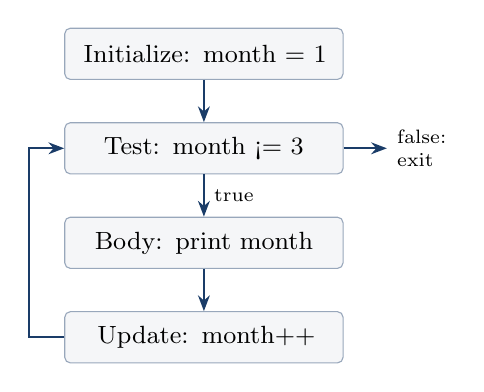
\begin{tikzpicture}[stage/.style={draw=BootcampBlueDark!45,fill=SoftGray,
  rounded corners=2pt,text width=3.3cm,minimum height=0.65cm,align=center,font=\small},
  flow/.style={-{Stealth[length=2mm]},thick,draw=BootcampBlueDark}]
\node[stage] (init) at (0,3.6) {Initialize: month = 1};
\node[stage] (test) at (0,2.4) {Test: month <= 3};
\node[stage] (body) at (0,1.2) {Body: print month};
\node[stage] (update) at (0,0) {Update: month++};
\draw[flow] (init) -- (test);
\draw[flow] (test) -- node[right,font=\scriptsize]{true} (body);
\draw[flow] (body) -- (update);
\draw[flow] (update.west) -- ++(-0.45,0) |- (test.west);
\draw[flow] (test.east) -- ++(0.55,0) node[right,font=\scriptsize,align=left]{false:\\exit};
\end{tikzpicture}
\end{column}
\end{columns}
\end{frame}

% 10 -- 1 min.
\begin{frame}{Increment and decrement: update, then consider the value}
\relax
\intro{These operators change an integer by one. Prefix/postfix matters when their value is used.}
\renewcommand{\arraystretch}{1.3}
\begin{tabularx}{\textwidth}{@{}l l X@{}}
\toprule
\textbf{Expression} & \textbf{Change to i} & \textbf{Value supplied by the expression} \\
\midrule
\texttt{i++} & Add 1 & The old value, before the increment. \\
\texttt{++i} & Add 1 & The new value, after the increment. \\
\texttt{i--} & Subtract 1 & The old value, before the decrement. \\
\texttt{--i} & Subtract 1 & The new value, after the decrement. \\
\bottomrule
\end{tabularx}\par
\begin{definitionblock}{In the update part of a for loop}
\raggedright
The expression's value is unused. Replacing \texttt{i++} with \texttt{++i}
there gives the same traversal. A backward traversal typically uses \texttt{i--}.
\end{definitionblock}
{\small Example: starting with i = 4, \texttt{int previous = i++;} leaves previous = 4 and i = 5.}
\end{frame}

% 11 -- 1.5 min.
\begin{frame}[fragile]{Nested loops express two levels of repetition}
\relax
\intro{One outer iteration runs the entire inner loop. Here n selects a tree row and i selects a node.}
\begin{columns}[T,onlytextwidth]
\begin{column}{0.51\textwidth}
\begin{lstlisting}
const int N = 2;
for (int n = 0; n <= N; n++)
{
    for (int i = 0; i <= n; i++)
    {
        // Work on node (n, i).
    }
}
\end{lstlisting}
\end{column}
\begin{column}{0.45\textwidth}
\renewcommand{\arraystretch}{1.5}
\begin{tabular}{@{}cl@{}}
\textbf{Row} & \textbf{Nodes visited} \\
0 & \texttt{(0,0)} \\
1 & \texttt{(1,0), (1,1)} \\
2 & \texttt{(2,0), (2,1), (2,2)}
\end{tabular}
\medskip\par
The inner counter restarts at zero for each row. Its upper bound depends on the current n.
\end{column}
\end{columns}
\begin{propositionblock}{Match the loop bounds to the structure}
\raggedright
Row n has n + 1 nodes, numbered 0 through n. These bounds follow the shape of the tree.
\end{propositionblock}
\end{frame}

% 12 -- 1.5 min.
\begin{frame}[fragile]{An array stores several values under one name}
\relax
\intro{An array contains a fixed number of elements of the same type, stored contiguously.}
\begin{lstlisting}
const int SIZE = 4;
double prices[SIZE] = {98.0, 101.0, 99.0, 104.0};
\end{lstlisting}
\begin{center}
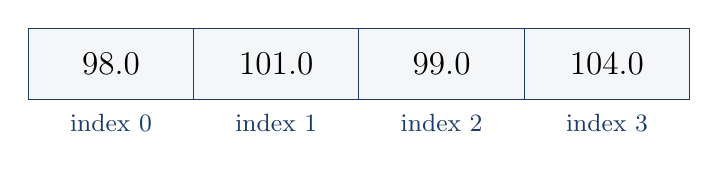
\begin{tikzpicture}[cell/.style={draw=BootcampBlueDark,fill=SoftGray,
 minimum width=2.1cm,minimum height=0.9cm,font=\large}]
\foreach \idx/\val in {0/98.0,1/101.0,2/99.0,3/104.0} {
 \node[cell] at (2.1*\idx,0) {\val};
 \node[font=\small,text=BootcampBlueDark] at (2.1*\idx,-0.75) {index \idx};
}
\end{tikzpicture}
\end{center}
\textbf{Size is a count; an index is a position.}\par
There are four elements. The first is \texttt{prices[0]}; the last is \texttt{prices[3]}.
\begin{illustrationblock}{The valid range is 0 <= index < SIZE}
\raggedright
Raw array indexing does not check bounds. Accessing \texttt{prices[SIZE]} is outside this array and has undefined behavior.
\end{illustrationblock}
\end{frame}

% 13 -- 1 min.
\begin{frame}[fragile]{Initialize an array, then traverse its valid indices}
\relax
\intro{Inside main(). This fixed-size style follows the course examples.}
\begin{lstlisting}
const int SIZE = 4;
double prices[SIZE] = {0.0};
for (int i = 0; i < SIZE; i++)
{
    prices[i] = 100.0 + i;
}
\end{lstlisting}
\begin{columns}[T,onlytextwidth]
\begin{column}{0.48\textwidth}
\begin{definitionblock}{After initialization}
\raggedright
\texttt{[0.0, 0.0, 0.0, 0.0]}\par
The first initializer is explicit; the remaining double elements are zero-initialized.
\end{definitionblock}
\end{column}
\begin{column}{0.48\textwidth}
\begin{propositionblock}{After the loop}
\raggedright
\texttt{[100.0, 101.0, 102.0, 103.0]}\par
Each valid element receives one value. The condition excludes index SIZE.
\end{propositionblock}
\end{column}
\end{columns}
\end{frame}

% 14 -- 1 min, optional extension.
\begin{frame}[fragile]{Optional extension: a vector can change its size}
\relax
\intro{Include <vector>. std::vector<double> denotes a sequence of doubles.}
\begin{lstlisting}
// Inside main():
std::vector<double> prices = {100.0, 102.0};
prices.push_back(101.0);
\end{lstlisting}
\begin{definitionblock}{What changed}
\raggedright
\texttt{push\_back} appends one element: the sequence is now \texttt{[100.0, 102.0, 101.0]}.\par
\texttt{prices.size()} reports three elements. Existing elements keep their positions.
\end{definitionblock}
\textbf{Indexing still starts at zero.}\par
Valid indices are smaller than \texttt{size()}; \texttt{operator[]} does not automatically check bounds.
\medskip\par
{\small Use the course's fixed-size arrays for now. This type also illustrates how a function can receive a larger collection of values.}
\end{frame}

% 15 -- 1.5 min.
\begin{frame}[fragile]{A function packages a calculation behind a name}
\relax
\intro{A caller supplies arguments; parameters receive them; return supplies the result.}
\begin{lstlisting}
double Discount(double amount, double factor)
{
    return amount / factor;
}
// Inside main(); assume factor > 0:
double presentValue = Discount(105.0, 1.05);
\end{lstlisting}
\begin{center}
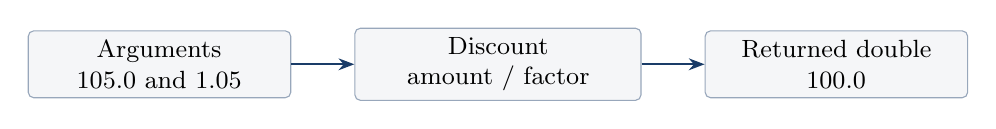
\begin{tikzpicture}[box/.style={draw=BootcampBlueDark!45,fill=SoftGray,
 rounded corners=2pt,minimum height=0.85cm,align=center,font=\small},
 flow/.style={-{Stealth[length=2mm]},thick,draw=BootcampBlueDark}]
\node[box,text width=3.1cm] (args) {Arguments\\105.0 and 1.05};
\node[box,text width=3.4cm,right=0.8cm of args] (calc) {Discount\\amount / factor};
\node[box,text width=3.1cm,right=0.8cm of calc] (result) {Returned double\\100.0};
\draw[flow] (args) -- (calc);
\draw[flow] (calc) -- (result);
\end{tikzpicture}
\end{center}
\textbf{The return type describes the result; the parameter types describe the inputs.}\par
{\small A return statement ends this function call. Its result can initialize a variable or become part of another expression.}
\end{frame}

% 16 -- 1 min.
\begin{frame}[fragile]{A declaration describes the interface; a definition supplies the body}
\relax
\begin{definitionblock}{Declaration: what a caller needs to know}
\begin{lstlisting}
double Discount(double amount, double factor);
\end{lstlisting}
\raggedright
The signature tells the caller which arguments to supply and which result to expect.
A declaration ends with a semicolon and has no body.
\end{definitionblock}
\begin{propositionblock}{Definition: how the function does its work}
\begin{lstlisting}
double Discount(double amount, double factor)
{
    return amount / factor;
}
\end{lstlisting}
\raggedright
The braces contain the implementation. Its signature must match the declaration.
\end{propositionblock}
\end{frame}

% 17 -- 1 min.
\begin{frame}[fragile]{Namespaces group names and make their origin explicit}
\relax
\intro{The course uses fre for its own functions and std for standard-library facilities.}
\begin{lstlisting}
namespace fre
{
    double Discount(double amount, double factor);
}
\end{lstlisting}
\renewcommand{\arraystretch}{1.3}
\begin{tabularx}{\textwidth}{@{}l X@{}}
\toprule
\textbf{Qualified name} & \textbf{How to read it} \\
\midrule
\texttt{fre::Discount} & Discount in the course's fre namespace. \\
\texttt{std::cout} & cout in the standard-library namespace std. \\
\texttt{std::pow} & pow in std; its declaration is available through <cmath>. \\
\bottomrule
\end{tabularx}\par
\medskip
\textbf{\texttt{::} selects a name from a scope.}\par
Namespaces allow different groups of code to use the same short names.
Use explicit \texttt{std::} and \texttt{fre::} in these examples.
\end{frame}

% 18 -- 1.5 min. Full header/definition, continued with caller on slide 19.
\begin{frame}[fragile]{Headers share declarations; source files define functions}
\relax
\intro{The header is included wherever its declarations are needed, including in its implementation file.}
\begin{columns}[T,onlytextwidth]
\begin{column}{0.46\textwidth}
\textbf{Finance.h}
\begin{lstlisting}
#pragma once
namespace fre
{
double Discount(double amount,
                double factor);
}
\end{lstlisting}
\medskip
\texttt{\#pragma once} prevents repeated inclusion of this header within one compilation unit.
\end{column}
\begin{column}{0.50\textwidth}
\textbf{Finance.cpp}
\begin{lstlisting}
#include "Finance.h"
namespace fre
{
double Discount(double amount,
                double factor)
{
    return amount / factor;
}
}
\end{lstlisting}
\end{column}
\end{columns}
\smallskip
\textbf{Keep the same namespace and signature in both files.}\par
{\small This separation lets several source files call a function through a shared declaration.}
\end{frame}

% 19 -- 1.5 min.
\begin{frame}[fragile]{Building the program connects calls to definitions}
\relax
\begin{columns}[T,onlytextwidth]
\begin{column}{0.49\textwidth}
\textbf{Main.cpp}
\begin{lstlisting}
#include "Finance.h"
#include <iostream>
int main()
{
    double pv = fre::Discount(
        105.0, 1.05);
    std::cout << pv << std::endl;
    return 0;
}
\end{lstlisting}
\end{column}
\begin{column}{0.47\textwidth}
\textbf{1. Include the declaration.}\par
Main.cpp can check the argument and result types.
\medskip\par
\textbf{2. Compile the source files.}\par
Each \texttt{.cpp} file is translated separately.
\medskip\par
\textbf{3. Link the program.}\par
The definition in Finance.cpp supplies the function called by Main.cpp.
\end{column}
\end{columns}
\begin{lstlisting}[language={}]
g++ Main.cpp Finance.cpp -o pricer
./pricer
\end{lstlisting}
{\small Build both .cpp files from this folder. Including Finance.h does not compile Finance.cpp.}
\end{frame}

% 20 -- 1.5 min.
\begin{frame}[fragile]{Pass by value gives a function its own copy}
\relax
\begin{columns}[T,onlytextwidth]
\begin{column}{0.49\textwidth}
\begin{lstlisting}
double AddFee(double amount)
{
    amount = amount + 2.0;
    return amount;
}
// Inside main():
double cash = 100.0;
double total = AddFee(cash);
\end{lstlisting}
\end{column}
\begin{column}{0.47\textwidth}
\begin{definitionblock}{Two independent variables}
\raggedright
The parameter amount starts with a copy of cash's value.
Changing amount does not change cash.
\end{definitionblock}
\textbf{After the call}\par
\texttt{cash = 100.0}\par
\texttt{total = 102.0}
\end{column}
\end{columns}
\begin{center}
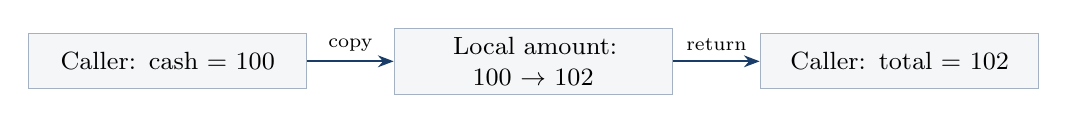
\begin{tikzpicture}[box/.style={draw=BootcampBlueDark!40,fill=SoftGray,
 text width=3.3cm,minimum height=0.7cm,align=center,font=\small},
 flow/.style={-{Stealth[length=2mm]},thick,draw=BootcampBlueDark}]
\node[box] (caller) {Caller: cash = 100};
\node[box,right=1.1cm of caller] (copy) {Local amount: 100 $\to$ 102};
\node[box,right=1.1cm of copy] (result) {Caller: total = 102};
\draw[flow] (caller) -- node[above,font=\scriptsize]{copy} (copy);
\draw[flow] (copy) -- node[above,font=\scriptsize]{return} (result);
\end{tikzpicture}
\end{center}
\end{frame}

% 21 -- 1.5 min. This is an alternative function, not combined with slide 20.
\begin{frame}[fragile]{Pass by reference gives another name to the caller's variable}
\relax
\intro{Alternative implementation: the ampersand changes the relationship between parameter and argument.}
\begin{columns}[T,onlytextwidth]
\begin{column}{0.49\textwidth}
\begin{lstlisting}
void AddFee(double& amount)
{
    amount = amount + 2.0;
}
// Inside main():
double cash = 100.0;
AddFee(cash);
\end{lstlisting}
\end{column}
\begin{column}{0.47\textwidth}
\begin{propositionblock}{One variable, two names}
\raggedright
amount is an alias for cash during this call.
Assigning through amount updates cash itself.
\end{propositionblock}
\textbf{After the call: \texttt{cash = 102.0}.}\par
The return type void means this call produces no returned value.
\end{column}
\end{columns}
\medskip
\centering
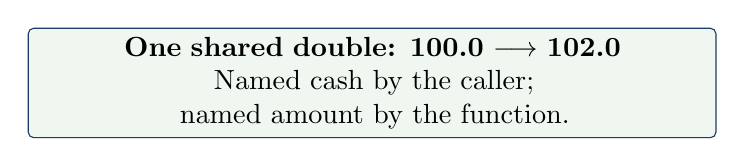
\begin{tikzpicture}
\node[draw=BootcampBlueDark,fill=MatrixGreen!7,rounded corners=2pt,
 text width=8.5cm,align=center,minimum height=1cm]
 {\textbf{One shared double: 100.0 $\longrightarrow$ 102.0}\\
 Named cash by the caller; named amount by the function.};
\end{tikzpicture}
\end{frame}

% 22 -- 1.5 min. Scalar const reference follows Topic 2; vector note optional.
\begin{frame}[fragile]{A const reference allows reading through an alias}
\relax
\begin{lstlisting}
bool IsPositive(const double& value)
{
    return value > 0.0;
}
\end{lstlisting}
\begin{definitionblock}{Two separate promises in the parameter type}
\raggedright
\texttt{\&}: value refers to the caller's object instead of holding a separate copy.\par
\texttt{const}: the function cannot modify that object through value.
An assignment to value, or \texttt{value++}, would be rejected.
\end{definitionblock}
\textbf{The caller's own non-const variable can still change later.}
\par
{\small\textbf{Optional collection example:} a const reference avoids copying a whole vector while allowing the function to read its elements.}
\begin{lstlisting}
double Total(const std::vector<double>& prices);
\end{lstlisting}
\end{frame}

% 23 -- 1 min.
\begin{frame}{Choose parameter types from the function's job}
\relax
\intro{First decide whether the function must change the caller's object. Then consider copying.}
\renewcommand{\arraystretch}{1.4}
\begin{tabularx}{\textwidth}{@{}p{3.5cm} p{3.4cm} X@{}}
\toprule
\textbf{Job} & \textbf{Parameter style} & \textbf{Reason} \\
\midrule
Read a small number & \texttt{double amount} & A cheap copy; the caller is unaffected. \\
Update the caller & \texttt{double\& amount} & Assignments change the original variable. \\
Read a larger object & \texttt{const T\& object} & Avoid a copy; prevent writes through this parameter. \\
\bottomrule
\end{tabularx}\par
\smallskip
{\small Here T is shorthand for a type such as \texttt{std::vector<double>} (optional extension).}
\begin{propositionblock}{The lecture's const double references are valid}
\raggedright
For a simple double used only as input, passing by value is usually sufficient.
A const reference matters more when copying a larger object would be costly.
\end{propositionblock}
\end{frame}

% 24 -- 1.5 min.
\begin{frame}[fragile]{The CRR loop combines familiar building blocks}
\relax
\intro{Price initially holds N + 1 terminal payoffs. Assume N >= 1, R > 0, and 0 < q < 1.}
\begin{columns}[T,onlytextwidth]
\begin{column}{0.57\textwidth}
\begin{lstlisting}
for (int n = N - 1; n >= 0; n--)
{
    for (int i = 0; i <= n; i++)
    {
        Price[i] =
            (q * Price[i + 1]
             + (1.0 - q) * Price[i]) / R;
    }
}
\end{lstlisting}
\end{column}
\begin{column}{0.39\textwidth}
\textbf{Outer loop: move backward in time.}\par
Terminal values at N are known; compute rows N - 1 through 0.
\medskip\par
\textbf{Inner loop: visit the current row.}\par
Row n contains nodes 0 through n. Each needs children i and i + 1.
\end{column}
\end{columns}
\smallskip
\textbf{Before an assignment:} the two array entries hold next-step option values.\par
\textbf{After it:} Price[i] holds the current node's value. After all rows, Price[0] is today's value.
\smallskip\par
{\small The signed int n can become -1 to end the loop; the largest child index is N, inside the N + 1 slots.}
\end{frame}

% 25 -- 1.5 min. Worked illustration, no prediction/reveal.
\begin{frame}{Updating in place reuses memory while preserving needed values}
\relax
\intro{One worked row: n = 1, q = 0.5, R = 1.0. Each parent is the average of its two children.}
\renewcommand{\arraystretch}{1.45}
\begin{tabularx}{\textwidth}{@{}l c c c X@{}}
\toprule
\textbf{Stage} & \textbf{Slot 0} & \textbf{Slot 1} & \textbf{Slot 2} & \textbf{What happens} \\
\midrule
Before the loop & 2 & 4 & 8 & All three entries are next-step values. \\
After i = 0 & \textcolor{MatrixGreen}{\textbf{3}} & 4 & 8 & Read 2 and 4, then overwrite slot 0. \\
After i = 1 & \textcolor{MatrixGreen}{\textbf{3}} & \textcolor{MatrixGreen}{\textbf{6}} & \textcolor{gray}{8} & Read 4 and 8, then overwrite slot 1. \\
\bottomrule
\end{tabularx}\par
\begin{propositionblock}{The new active row is [3, 6]}
\raggedright
Moving left to right leaves both required children untouched until they are read.
Slot 2 remains allocated, but is no longer part of the active row.
\end{propositionblock}
{\small Reversing the inner loop would reuse an already updated child.
Traversal order is part of the algorithm's correctness.}
\end{frame}

% 26 -- 1.5 min.
\begin{frame}{Count the repeated work to understand complexity}
\relax
\intro{For the backward CRR loop, each node update uses a constant number of arithmetic operations.}
\begin{columns}[T,onlytextwidth]
\begin{column}{0.48\textwidth}
\begin{definitionblock}{Time: count node updates}
\raggedright
Rows contain N, N - 1, \ldots, 1 active nodes:
\[
N+(N-1)+\cdots+1=\frac{N(N+1)}{2}.
\]
For large N, doubling N roughly quadruples the work: \textbf{$O(N^2)$ time}.
\end{definitionblock}
\end{column}
\begin{column}{0.48\textwidth}
\begin{propositionblock}{Space: count stored values}
\raggedright
One array holds N + 1 values and is reused for each row.\par
\medskip
Doubling N roughly doubles storage: \textbf{$O(N)$ space}.
\end{propositionblock}
\end{column}
\end{columns}
\textbf{Big-O describes growth as the input size increases.}\par
{\small It is not a timing in seconds. This count covers the backward loop, not all setup or input/output work.}
\end{frame}

% 27 -- 0.5 min.
\begin{frame}{A reading guide for the practice deck}
\relax
\intro{Read a short program in this order, then explain how its values change.}
\renewcommand{\arraystretch}{1.35}
\begin{tabularx}{\textwidth}{@{}l X@{}}
\toprule
\textbf{Look at} & \textbf{Establish} \\
\midrule
Types and initializers & What each variable can store and its starting value. \\
Expressions and conditions & Operand types, calculation order, and the chosen path. \\
Loop headers & Start, stopping condition, and update after each iteration. \\
Array indices & Which elements exist and which values are still needed. \\
Function parameters & Whether the function receives a copy or an alias. \\
Return statements & What value the caller receives, if any. \\
Headers and source files & Where a name is declared and where its body is defined. \\
\bottomrule
\end{tabularx}\par
\medskip
\textbf{Now apply these ideas independently in Deck 4.}
\end{frame}

\end{document}
